\documentclass{VUMIFPSkursinis}
\usepackage{algorithmicx}
\usepackage{algorithm}
\usepackage{algpseudocode}
\usepackage{amsfonts}
\usepackage{amsmath}
\usepackage{bm}
\usepackage{caption}
\usepackage{color}
\usepackage{float}
\usepackage{graphicx}
\usepackage{listings}
\usepackage{subfig}
\usepackage{wrapfig}

% Titulinio aprašas
\university{Vilniaus universitetas}
\faculty{Matematikos ir informatikos fakultetas}
\institute{Informatikos institutas}  % Užkomentavus šią eilutę - institutas neįtraukiamas į titulinį
\department{Programų sistemų studijų programa}
\papertype{Kursinis darbas}
\title{Vaizdo žaidimo eismo vaizdų generavimas naudojant nesuporuotų nuotraukų vertimą}
\titleineng{Video game traffic image generation using unpaired image to image translation}
\status{4 kurso 5 grupės studentas}
\author{Gytis Oksas}
\supervisor{j. asist. Boleslovas Dapkūnas}
\date{Vilnius – \the\year}

% Nustatymai
% \setmainfont{Palemonas}   % Pakeisti teksto šriftą į Palemonas (turi būti įdiegtas sistemoje)
\bibliography{bibliografija}

\begin{document}
\maketitle

\tableofcontents

\sectionnonum{Įvadas}
    Paveikslėlio vertimas kitu paveikslėliu (angl. image-to-image (I2I) translation) yra plačiai taikoma metodika kompiuterių regos ir paveikslų apdorojimo problemoms spręsti \cite{ImTImTr}. Metodai, sprendžiantys šias problemas, gali būti taikomi parinktų specifinių paveikslėlių požymių keitimui, trūkstamų paveikslėlio pikselių užpildymui arba realistinių vaizdų generavimui. Šiame darbe pristatomas naujas įrankis generuoti žaidimo eismo vaizdus iš realistinių eismo vaizdų. Ši taikymo sritis gali būti naudinga kuriant žaidimų meninį turinį (pavyzdžiui, tekstūras, realistinių objektų dizaino atitikmenis žaidimui), kuriant animacijas. Ir nors realistinių vaizdų transformavimas į nerealistinių vaizdų domeną nėra naujas (pavyzdžiui, veido nuotraukas transformuoti į animacinių filmukų stilių), kelių eismo nuotraukų transformavimas į vaizdo žaidimų domeną yra labai mažai nagrinėtas.
    
    Šio tyrimo tikslas ir yra - sukurti modelį, kuris generuotų tam tikro žaidimo vaizdus iš jų norimo realistinio atitikmens, šiame tyrime buvo pasirinkta kurti žaidimo „Grand Theft Auto: Vice City" (toliau trumpinama „GTA:VC") domeną dėl jo išskirtinio meninio stiliaus ir ryškaus domeno požymių skirtumo lyginant su realaus eismo nuotraukomis.
    
    Tyrimo tikslas yra sukurti modelį, kuris pasiektų FID įvertį žemesnį nei 100, vizualiai būtų kuo panašesnis į žaidimų vaizdus ir išsaugotų kuo daugiau tikrų nuotraukų detalių.
\section{Literatūra ir kiti tyrimai}
    \subsection{Žaidimų vaizdai į realybės vaizdus}
        Tyrimas kuris atkreipė daug dirbtinio intelekto ir vaizdo žaidimų mėgėjų dėmesį yra aprašytas Intel dirbtinio intelekto mokslininkų straipsnyje "Enhancing Photorealism Enhancement" \cite{EnPhEn}, kuriame pasakojama, kaip išnaudojus modernias dirbtinio intelekto technologijas yra sukuriamas nuotraukų transformatoriaus modelis, sugebantis žaidimo GTA V automobilių eismo vaizdus paversti foto realistiniais, lyg įrašytais automobilio registratoriumi. Jis vienas pirmųjų įtikinamai, švariai, be prarastų esminių nuotraukų detalių ir be pridėtinių artefaktų sugebėjo transformuoti nuotrauką į realistiškai atrodantį vaizdą (žr. 1 pav.). Tai davė idėją šiam tyrimui - apsukti puses ir sukurti modelį, kuris pagal tuos pačius atributus sugebėtų transformuoti realybės automobilių eismo vaizdus į vaizdo žaidimo automobilių eismo vaizdus.
        \begin{figure}[H]
            \centering
            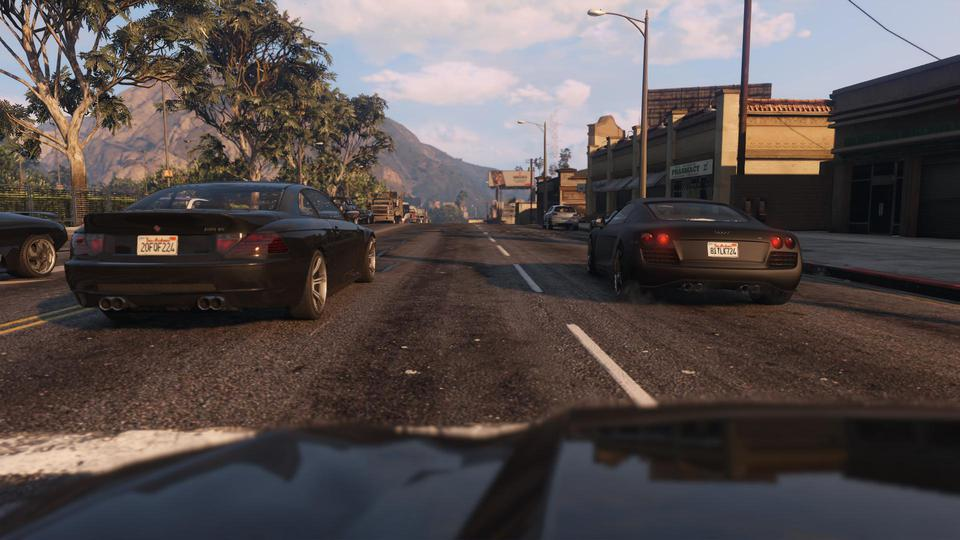
\includegraphics[scale=0.25]{img/EnPhEn_before}
            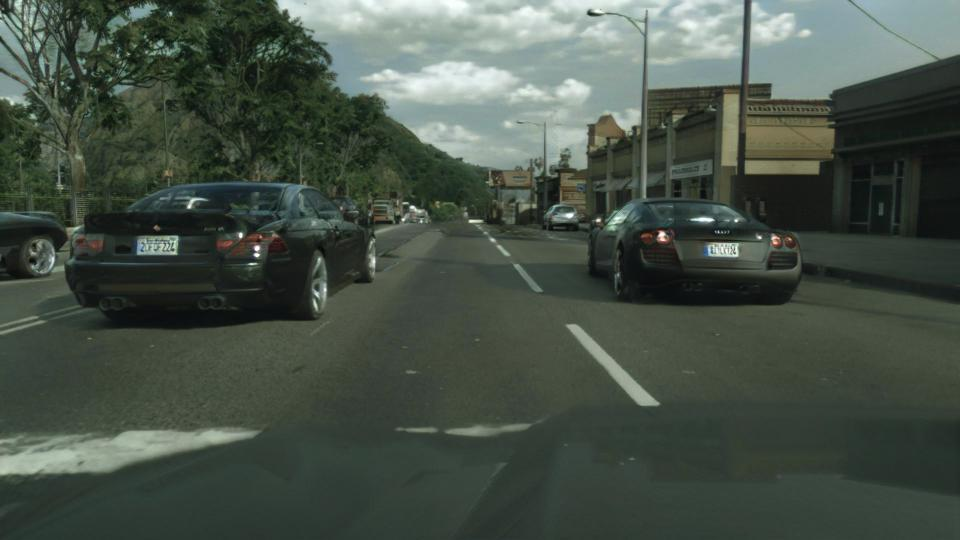
\includegraphics[scale=0.25]{img/EnPhEn_after}
            \caption{Vaizdai prieš ir po nuotraukos transformavimo, atitinkamai.\cite{EnPhEn}}
            \label{img:mlp}
        \end{figure}
    \subsection{CycleGAN modelis}
        Vienas iš trijų panaudotų nuotraukų transformavimo modelių yra CycleGAN modelis \cite{CycleGAN2017}, sukurtas 2017 metais, tačiau išpopuliarėjęs savo galimybe vaizdus transformuoti į abi puses, t.y. modelį išmokius nuotraukas transformuoti iš domeno A į domeną B, jis taip pat sugebės vaizdus transformuoti iš domeno B į domeną A, nors nebūtinai taip pat gerai.

        Tyrimo straipsnyje yra vaizduojama, kaip modelis sugeba transformuoti vaizdus tarp realistinių domenų (pavyzdžiui, iš arklio į zebrą ir iš zebro į arklį) ir tarp nerealistinių ir realistinių (pavyzdžiui, iš kraštovaizdžio nuotraukų į Monet paveikslus ir atvirškčiai). Tarp dviejų nerealistinių domenų pavyzdžių nėra, tačiau galima nuspėti, jog su kokybišku apmokymo procesu ir duomenų rinkiniu tokį uždavinį taip pat nesunkiai įveiktų.

        Nors modelis jau lygintinai dirbtinio intelekto pasaulyje yra senas, tačiau dėl jo kodo realizacijos prieinamumo ir architektūros paprastumo yra vertas dėmesio ir laiko.
        
    \subsection{CUT modelis}
        Antras iš trijų naudotų modelių yra CUT (pilnas angliškas pavadinimas - contrastive unpaired translation), išleistas 2020 metais. Pagrindinis jo bruožas yra, jog jis yra pritaikytas mokymui su nesuporuotomis nuotraukomis (t.y. nuotraukai iš domeno A, nėra tiesioginio atitikmens iš domeno B). Kitaip nei CycleGAN, CUT mokymas ir nuotraukų transformavimas vykdomas tik į vieną pusę, tai reiškia, kad norint nuotraukas transformuoti iš domeno A į domeną B ir iš domeno B į domeną A, yra reikalingi du atskirai išmokyti modeliai. Dėl vienpusio nuotraukų transformavimo, mokymo procedūra yra supaprastinama ir paspartinama. Šio modelio tikslas yra transformuojant perimti norimo domeno išvaizdą, bet išlaikyti transformuojamos nuotraukos struktūrą ir esminį turinį. Būtent ši CUT modelio savybė ir pakiša koją transformuojant nuotraukas kai kuriuose domenuose, kadangi jei apmokant modelį yra dažnai pasitaikančių artefaktų, tai jie gali dažnai atsikartoti ir transformuojamose nuotraukose, tai yra pabrėžiama "Enhancing Photorealism Enhancement" \cite{EnPhEn} straipsnyje, kur transformuojant GTA V vaizdus, CUT modelis dažnai ant žaidėjo automobilio variklio dangčio uždėdavo Mercedes žvaigždę, kuri beveik visados matoma Cityscapes duomenų rinkinyje \cite{DaimCityDaSe}, kuriuo ir buvo mokinti modeliai.
    \subsection{MSPC modelis}
        Trečiasis naudotas modelis yra MSPC (pilnas pavadinimas angliškai - Maximum Spatial Perturbation Consistency) \cite{Mspc}. Jis yra sukurtas CycleGAN \cite{CycleGAN2017} pagrindu, todėl jo nuotraukų transformavimas taip pat yra komutatyvus. Šis modelis yra sukurtas su tikslu jį naudoti nesuporuotų nuotraukų duomenų rinkiniams, kurie dažnai priveda prie nuotraukos turinio išdarkymo. Būtent šią problemą MSPC modelis ir bando spręsti, bandant geriau išsaugoti turinio bruožus ir jų turinį. 
\section{Metodologija}
    \subsection{Duomenų rinkiniai}
        \subsubsection{Naudojami duomenų rinkiniai}
            Vaizdų transformavimui iš realistinių į GTA:VC vaizdus reikėjo dviejų duomenų rinkinių: realaus eismo vaizdų ir žaidimo eismo vaizdų. Realaus eismo vaizdų duomenų rinkinių yra pakankamai daug, todėl jų rinkti nereikėjo ir buvo pasirinktas bdd100k rinkinys, o GTA:VC vaizdams reikėjo kurti savo duomenų rinkinį, kadangi kokybiško ir kiekybiško rinkinio internete rasti nepavyko. 
        \subsubsection{Realistinių vaizdų duomenų rinkinys}
            Kaip minėta, buvo naudojamas bdd100k duomenų rinkinys. Jis sudarytas iš 100 tūkst. automobilių eismo nuotraukų, padarytų naudojant kameras nukreiptas į automobilio važiavimo kryptį ir yra dažniausiai ant automobilio priekinės panelės. Buvo naudotas jo poaibis sudarytas iš 10 tūkst. nuotraukų, kadangi GTA:VC nuotraukų duomenų rinkinys gavosi lygintinai mažas. 10 tūkst. nuotraukų duomenų rinkinys yra padalintas 70:20:10 santykiu mokymui, testavimui ir validacijai (atitinkamai gaunasi 7 tūkst, 2 tūkst ir 1 tūkst). Kiekviena nuotrauka yra 1280:720 pikselių raiškos.

            Papildomo apdorojimo ar modifikacijų duomenų rinkiniui nereikėjo, išskyrus paprasčiausią direktorijų keitimą ir aplankų pervadinimą, jog modelio treniravimo algoritmas žinotų, kur tiksliai rasti šaltinio domeno duomenų rinkinį.
        \subsubsection{Grand Theft Auto: Vice City duomenų rinkinys}
            Eksperimentą daryti buvo norima su GTA:VC vaizdais, tačiau jo duomenų rinkinio internete rasti nepavyko, todėl teko jį sukurti. Džiugu, jog kokybišką ir kiekybišką duomenų rinkinį leido sukurti žaidimo grafiniai nustatymai, todėl papildomų modifikacijų į žaidimą diegti nereikėjo, vienintelis dalykas, ko prireikė - ekrano vaizdo įrašymo programinės įrangos. Ekrano vaizdo įrašymui naudojama buvo OBS Studio programa.
            
            OBS Studio programos paruošimo nereikėjo, bet buvo pakeistos kelios parinktys, kad kuriamas duomenų rinkinys būtų struktūriškai kuo panašesnis į šaltinio duomenų rinkinį ir vaizdo įrašai nesigautų be reikalo dideli ir sunkūs apdoroti. Pirma pakeista parinktis buvo pakeista raiška į bdd100k rinkinio nuotraukų raišką (kuri yra 1280:720 pikselių). Antras pakeitimas buvo nustatyti vaizdo įrašų kadrų dažnį kiekį į 1 kadrą per sekundę. Su paskutine parinktimi supaprastiname vaizdo įrašų perdarymą į nuotraukas, nes nereikia išmesti perteklinių nuotraukų nustačius didesnį kadrų dažnį (pvz. nustačius standartinius 60 kadrų per sekundę, gautume žymiai per daug nuotraukų).
            
            GTA:VC žaidimui reikėjo kelių vaizdinių pakeitimų tam, kad būtų švaresni vaizdai ir būtų struktūriškai panašesnis į bdd100k duomenų rinkinį. Naudojant standartinius nustatymus yra rodomas vaizdas trečiuoju asmeniu (t.y. iš žaidėjo galo), apatiniame kairiajame kampe yra rodomas mažas žemėlapis ir viršuj dešinėje yra rodomi žaidimo duomenys: laikas, pinigai, gyvybės taškai, šarvų taškai, esami ginklai ir aktyvumas, kuriuo policija ieško žaidėjo (žr 2 pav.). Tam, kad vaizdas būtų artimesnis šaltinio domeno duomenų rinkiniui, reikėjo panaikinti žemėlapį ir informacines detales, tą žaidimas leido nustatymuose bei reikėjo nustatyti pirmą asmenį ir automobilio perspektyvos, kad nesimatytų pačio veikėjo ir taip išvengti nenorimų artefaktų (panašiai kaip įprastai lieka naudojant **dataset kur su mercedes** duomenų rinkinį, jame filmuojamas vaizdas iš automobilio Mercedes, o kadangi vaizduose yra matomas automobilio kapotas prie kurio pritvirtinta ikoniška Mercedes žvaigždė, todėl daugelyje transformuotų nuotraukų atsiranda minėtoji Mercedes žvaigždė). Šį pakeitimą žaidimas taip pat leidžia daryti, kaip konfiguracinį nustatymą. Šiuos pakeitimus implementavus, gaunamas kokybiškas ir švarus vaizdas, kuris nepalieka artefaktų ir užfiksuoja esminį turinį (žr. 3 pav.).
            
            \begin{figure}[H]
                \centering
                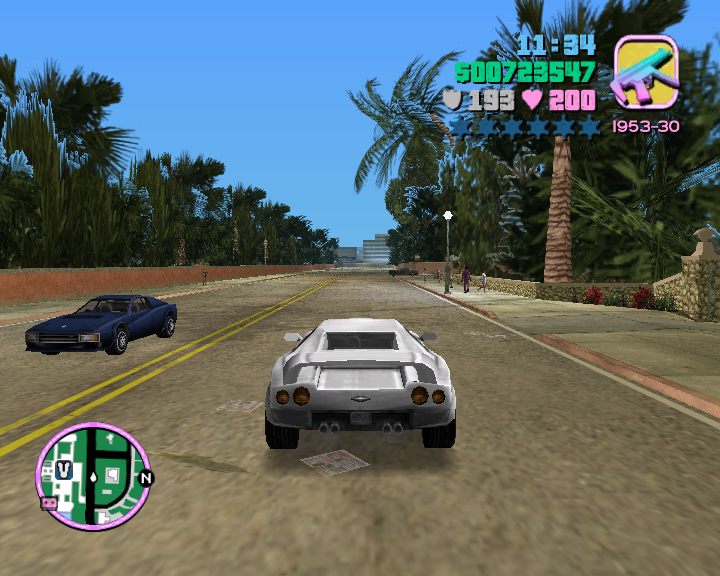
\includegraphics[scale=0.5]{img/neapdorotas_pvz}
                \caption{GTA:VC žaidimo vaizdas su įprastais nustatymais}
                \label{img:mlp}
            \end{figure}
            \begin{figure}[H]
                \centering
                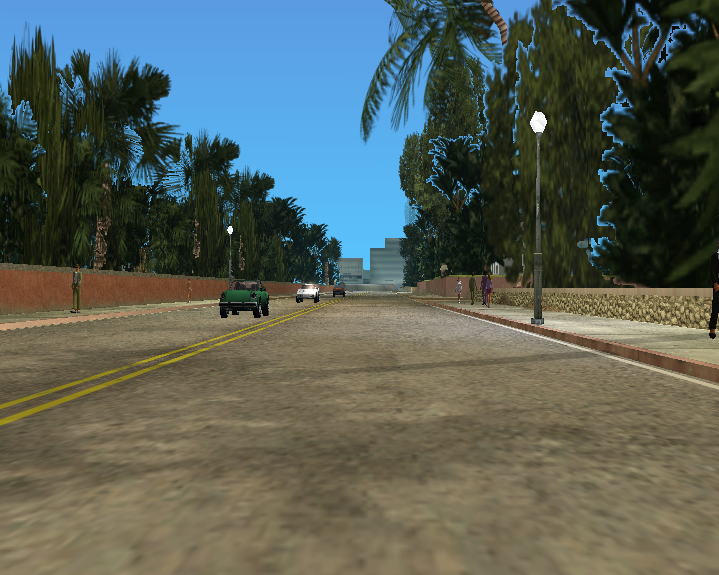
\includegraphics[scale=0.5]{img/apdorotas_pvz}
                \caption{GTA:VC žaidimo vaizdas su pakeistais nustatymais}
                \label{img:mlp}
            \end{figure}

            Duomenų rinkinio nuotraukos buvo kuriamos įrašinėjant GTA:VC žaidimo vaizdą, įrašuose važinėjant po žaidimo erdves keliais, bandant padengti kuo daugiau esamų vaizdų. Tas buvo daryta tiek žaidimo dienos metu, tiek nakties, kad būtų sukuriamas duomenų rinkinio aplinkybių vienodumas ir įvairumas. Žaidimo Pasaulis yra suskirstytas į 8 regionus. Kiekvienas regionas buvo išvažinėtas ir nufilmuotas žaidimo dienos ir nakties metu.
            
            Kitame skyriuje yra minima, jog rezultatuose yra pastebėta spragų - vaizdai turi žymiai mažiau automobilių nuotraukose nei bdd100k duomenų rinkinys, todėl po kelių eksperimentų, reikėjo papildyti surinktą duomenų rinkinį nuotraukomis, kuriuose yra daug automobilių arba jie užima didesnį ekrano plotą. Tokių nuotraukų iš viso buvo padaryta 300 ir jas pridėjus prie kitų nuotraukų buvo sukurta antra duomenų rinkinio versija.
            
            Visus regionus nufilmavus, jie buvo apdoroti Python kalbos skriptu, kuris vaizdo įrašo kadrus išskaidė į atskiras nuotraukas. Taip buvo iš viso sudaryta 2000 nuotraukų, o antra duomenų rinkinio versija buvo sudaryta iš 2300 nuotraukų.

        \subsection{Parinkti modeliai}
            Mokymui buvo išrinkti trys modeliai: CycleGAN, CUT ir MSPC.
        \subsection{Modelių mokymas}

\sectionnonum{Rezultatai ir išvados}

\sectionnonum{Santrumpos}
\begin{enumerate}
\item \textbf{GTA:VC} - Žaidimas „Grand Theft Auto: Vice City".
\item \textbf{GTA V} - Žaidimas „Grand Theft Auto 5".
\item \textbf{FID} - angliškai Fréchet inception distance, o lietuviškai Frečeto pradžios atstumas, yra metrika naudojama įvertinti generatyvinių modelių kokybę.
\end{enumerate}

\printbibliography[heading=bibintoc]

\end{document}
